%!TEX root = notes.tex

\chapter{Review of Optimization from Vector Calculus}\label{chapter:intro}

The starting point of these notes is the concept of \emph{optimization} as developed in MATH 241 (see e.g.~\cite[Chapter~14]{finney2001thomas})

\begin{definition}\label{def:localminimum}
Let $D\subseteq \field{R}^2$ be a region on the plane containing the point $(x_0, y_0)$.  We say that the real-valued function $f\colon D \to \field{R}$ has a \emph{local minimum} at $(x_0,y_0)$ if $f(x_0,y_0) \leq f(x,y)$ for all domain points $(x,y)$ in an open disk centered at $(x_0,y_0)$.  In that case, we also say that $f(x_0,y_0)$ is a \emph{local minimum value} of $f$ in $D$.
\end{definition}

Emphasis was made to find conditions on the function $f$ to guarantee existence and characterization of minima:

\begin{theorem}\label{theorem:localminimum}
Let $D \subseteq \field{R}^2$ and let $f \colon D \to \field{R}$ be a function for which first partial derivatives $\frac{\partial f}{\partial x}$ and $\frac{\partial f}{\partial y}$ exist in $D$.  If $(x_0,y_0) \in D$ is a local minimum of $f$, then $\gradient{f}(x_0,y_0)=0$.
\end{theorem}

The local minima of these functions are among the zeros of the equation $\gradient{f}(x,y)=0$, the so-called \emph{critical points} of $f$. More formally:

\begin{definition}\label{def:criticalpoint}
An interior point of the domain of a function $f(x,y)$ where both directional derivatives are zero, or where at least one of the directional derivatives do not exist, is a \emph{critical point} of $f$.
\end{definition}

We employed the \emph{Second Derivative Test for Local Extreme Values} to characterize some minima:
\begin{theorem}\label{theorem:2DTforLEV}
Suppose that $f\colon \field{R}^2 \to \field{R}$ and its first and second partial derivatives are continuous throughout a disk centered at the point $(x_0,y_0)$, and that $\gradient{f}(x_0,y_0)=0$. If the two following conditions are satisfied, then $f(x_0,y_0)$ is a local minimum value:
\begin{align}
\frac{\partial^2 f}{\partial x^2}(x_0,y_0) &> 0 \\
\det \underbrace{\begin{bmatrix} 
\dfrac{\partial^2 f}{\partial x^2}(x_0,y_0) & \dfrac{\partial^2 f}{\partial x \partial y}(x_0,y_0) \\ & \\
\dfrac{\partial^2 f}{\partial y \partial x}(x_0,y_0) & \dfrac{\partial^2 f}{\partial y^2}(x_0,y_0)
\end{bmatrix}}_{\Hess{f}(x_0,y_0)} &> 0
\end{align}
\end{theorem}

\begin{remark}
The restriction of this result to univariate functions is even simpler: Suppose $f''$ is continuous on an open interval that contains $x_0$.  If $f'(x_0)=0$ and $f''(x_0)>0$, then $f$ has a local minimum at $x_0$. 
\end{remark}

\begin{example}[Rosenbrock Functions]\label{example:Rosenbrock}
Given strictly positive parameters $a,b > 0$, consider the $(a,b)$--Rosenbrock function 
\begin{equation*} 
\mathcal{R}_{a,b}(x, y) = (a-x)^2 + b(y-x^2)^2.
\end{equation*}
It is easy to see that Rosenbrock functions are polynomials (prove it!).  The domain is therefore the whole plane. Figure \ref{figure:Rosenbrock} illustrates a contour plot with several level lines of $\mathcal{R}_{1,1}$ on the domain $D = [-2,2] \times [-1,3]$, as well as its graph.

\begin{figure}[ht!]
\begin{tabular}{cc}
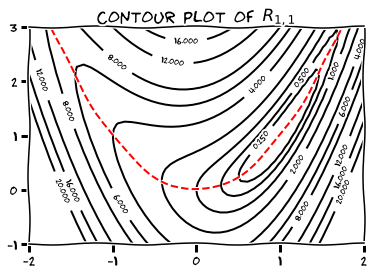
\includegraphics[width=0.5\linewidth]{rosenbrockContour} &
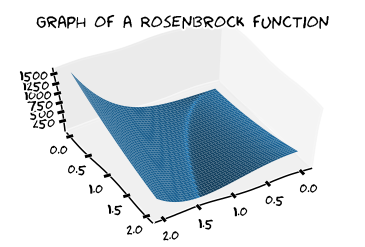
\includegraphics[width=0.5\linewidth]{rosenbrockGraph}
\end{tabular}
\caption{Details of the graph of $\mathcal{R}_{1,1}$}
\label{figure:Rosenbrock}
\end{figure}
It is also easy to verify that the image is the interval $[0,\infty)$.  Indeed, note first that $\mathcal{R}_{a,b}(x,y) \geq 0$ for all $(x,y) \in \field{R}^2$.  Zero is attained: $\mathcal{R}_{a,b} (a,a^2) = 0$.  Note also that $\mathcal{R}_{a,b}(0,y) = a^2 + by^2$ is a polynomial of degree 2, therefore unbounded.

Let's locate all local minima:
\begin{itemize}
	\item The gradient and Hessian are given respectively by
	\begin{equation*}
	\gradient{\mathcal{R}_{a,b}}(x,y) = \big[ 2(x-a) +4bx(x^2-y) , b(y-x^2) \big] \\
	\end{equation*}
	\begin{equation*}
	\Hess{\mathcal{R}_{a,b}}(x,y) = \begin{bmatrix}
	12bx^2-4by+2 & -4bx \\
	-4bx & 2b
	\end{bmatrix}
	\end{equation*}
	\item The search for critical points $\gradient{\mathcal{R}_{a,b}} = \boldsymbol{0}$ gives only the point $(a,a^2)$.
	\item $\frac{\partial^2 \mathcal{R}_{a,b}}{\partial x^2}(a,a^2) = 8ba^2+2 > 0$.
	\item The Hessian at that point has positive determinant:
	\begin{equation*}
	\det \Hess{\mathcal{R}_{a,b}}(a,a^2) = \det \begin{bmatrix}
	8ba^2+2 & -4ab \\
	-4ab & 2b
	\end{bmatrix} = 4b > 0
	\end{equation*}
\end{itemize}
There is only one local minimum at $(a,a^2)$.
\end{example}

The second step was the notion of \emph{global (or absolute) minima}: points $(x_0,y_0)$ that satisfy $f(x_0,y_0) \leq f(x,y)$ for any point $(x,y)$ in the domain of $f$.  We always started with the easier setting, in which we placed restrictions on the domain of our functions:

\begin{theorem}\label{theorem:MaxMinCompact}
A continuous real-valued function always attains its minimum value on a \emph{compact} set $K$. To search for global minima, we perform the following steps:
\begin{description}
	\item[Interior Candidates] List the critical points of $f$ located in the interior of $K$.
	\item[Boundary Candidates] List the points in the boundary of $K$ where $f$ may have minimum values.
	\item [Evaluation/Selection] Evaluate $f$ at all candidates and select the one(s) with the smallest value.
\end{description}
\end{theorem}

\begin{example}
A flat circular plate has the shape of the region $x^2+y^2 \leq 1$. The plate, including the boundary, is heated so that the temperature at the point $(x,y)$ is given by $f(x,y) =100(x^2 +2 y^2 - x)$ in Celsius degrees.  Find the temperature at the coldest point of the plate.

We start by searching for critical points.  The equation $\gradient{f}(x,y) = 0$ gives $x=\tfrac{1}{2}$, $y=0$. The point $(\tfrac{1}{2}, 0)$ is clearly inside of the plate.  This is our first candidate.

The border of the plate can be parameterized by $\varphi(t) = (\cos t, \sin t)$ for $t \in [0,2\pi)$.  The search for minima in the boundary of the plate can then be coded as an optimization problem for the function $h(t) = (f \circ \varphi) (t) = 100(\cos^2 t + 2\sin^2 t - \cos t)$ on the interval $[0,2\pi)$.  Note that $h'(t) = 0$ for $t \in \{ 0, \tfrac{2}{3}\pi \}$ in $[0,2\pi)$.  We thus have two more candidates: 
\begin{equation*}
\varphi(0) = (1,0) \qquad \varphi(\tfrac{2}{3}\pi)= \big( -\tfrac{1}{2}, \tfrac{1}{2}\sqrt{3} \big)
\end{equation*}
Evaluation of the function at all candidates gives us the solution to this problem: 
\begin{equation*}
f( \tfrac{1}{2}, 0 ) = -25^\circ\mathrm{C}.
\end{equation*}
\end{example}

On a second setting, we remove the restriction of boundedness of the function.  In this case, global minima will only be guaranteed for very special functions.

\begin{example}\label{example:CoerciveFunctions}
Any polynomial $p_n(x) = a_n x^n + a_{n-1} x^{n-1} + \dotsb + a_0$ with even degree $n \geq 2$ and positive leading coefficient satisfies 
$\lim_{\abs{x}\to \infty} p_n(x) = +\infty$.  
To see this, we may write
\begin{equation*}
a_n x^n + a_{n-1} x^{n-1} + \dotsb + a_0 = a_n x^n \big( 1 + \tfrac{a_{n-1}}{a_n x} + \dotsb + \tfrac{a_0}{a_n x^n} \big)
\end{equation*}
The behavior of each of the factors as the absolute value of $x$ goes to infinity leads to our claim.
\begin{align*}
\lim_{\abs{x} \to \infty} a_n x^n &= +\infty, \\
\lim_{\abs{x} \to \infty} \big( 1 + \tfrac{a_{n-1}}{a_n x} + \dotsb + \tfrac{a_0}{a_n x^n} \big) &= 1.
\end{align*}
It is clear that a polynomial of this kind must attain a minimum somewhere in its domain. The critical points will lead to them.
\end{example}

\begin{example}
Find the global minima of the function $f(x)= \log (x^4-2x^2+2)$ in $\field{R}$.  

Note first that the domain of $f$ is the whole real line, since $x^4-2x^2+2 = (x^2-1)^2+1 \geq 1$ for all $x\ \in \field{R}$.  Note also that we can write $f(x) = (g \circ h)(x)$ with $g(x) = \log(x)$ and $h(x)=x^4-2x^2+1$.  Since $g$ is one-to-one and increasing, we can focus on $h$ to obtain the requested solution.  For instance, $\lim_{\abs{x}\to\infty}f(x) = +\infty$, since $\lim_{\abs{x}\to\infty} h(x) = +\infty$. This guarantees the existence of global minima.  To look for it, $h$ again points to the possible locations by solving for its critical points: $h'(x)=0$.  We have then that $f$ attains its minima at $x=\pm 1$.
\begin{figure}[ht!]
\begin{center}
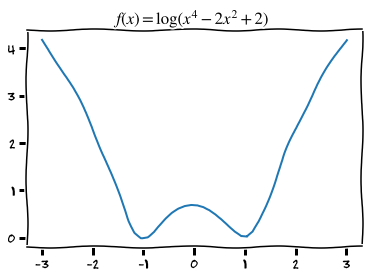
\includegraphics[width=0.5\linewidth]{coercivelog.png}
\end{center}
\caption{Global minima in unbounded domains}
\label{figure:coercivelog}
\end{figure}
\end{example}



\section{The Theory of Optimization}

The purpose of these notes is the development of a theory to deal with optimization in a more general setting.
\begin{itemize}
	\item We start in an Euclidean $d$--dimensional space with the usual topology based on the distance 
	\begin{equation*}
	\norm{\x-\y} = \langle \x-\y, \x-\y \rangle^{1/2} = \sqrt{\sum_{k=1}^d (x_k-y_k)^2 }.
	\end{equation*}
	\item Given a real-valued function $f\colon D \to \field{R}$ on a domain $D \subseteq \field{R}^d$, we define the concept of \emph{extrema}:
	\begin{definition}\label{def:extrema}
	Given a set $D \subseteq \mathbb{R}^d$, and a real-valued function $f\colon D \to \field{R}$, we say that a point $\xstar \in D$ is:
	\begin{enumerate}
		\item A \emph{global minimum} for $f$ on $D$ if $f(\xstar) \leq f(\x)$ for all $\x \in D$.
		\item A \emph{global maximum} for $f$ on $D$ if $f(\xstar) \geq f(\x)$ for all $\x \in D$.
		\item A \emph{strict global minimum} for $f$ on $D$ if $f(\xstar) < f(\x)$ for all $\x \in D \setminus \{ \xstar \}$.
		\item A \emph{strict global maximum} for $f$ on $D$ if $f(\xstar) > f(\x)$ for all $\x \in D \setminus \{ \xstar \}$.
		\item A \emph{local minimum} for $f$ on $D$ if there exists $\delta>0$ so that  $f(\xstar) \leq f(\x)$ for all $\x \in B_\delta(\xstar)\cap D$.
		\item A \emph{local maximum} for $f$ on $D$ if there exists $\delta>0$ so that  $f(\xstar) \geq f(\x)$ for all $\x \in B_\delta(\xstar)\cap D$.
		\item A \emph{local minimum} for $f$ on $D$ if there exists $\delta>0$ so that  $f(\xstar) < f(\x)$ for all $\x \in B_\delta(\xstar)\cap D$, $\x \neq \xstar$.
		\item A \emph{local maximum} for $f$ on $D$ if there exists $\delta>0$ so that  $f(\xstar) > f(\x)$ for all $\x \in B_\delta(\xstar)\cap D$, $\x \neq \xstar$.
	\end{enumerate}
	\end{definition}	
\end{itemize}
In this setting, the objective of \emph{optimization} is the following program:
\begin{description}
	\item[Existence of extrema] Establish results that guarantee the existence of extrema depending on the properties of $D$ and $f$. 
	\item[Characterization of extrema] Establish results that describe conditions for points $\x \in D$ to be extrema of $f$.  
	\item[Tracking extrema] Design robust numerical algorithms that find the extrema for scientific computing purposes. This is the core of these notes.  
\end{description}
The development of existence and characterization results will be covered in chapter \ref{chapter:existenceCharacterization}.  The design of algorithms to track extrema will be covered in chapter \ref{chapter:nonlinearoptimization}.